\chapter{原子核的基本性质}

核物理学科具有很广的覆盖度;
核物理的“唯象”特点;
重要的常数\& 常数组合;
合适的单位\& 相对论公式;
物质波(de Broglie, \nobel{1929}\footnote{由于核物理很多成就获得过20世纪Nobel奖,本笔记特标注了诺奖相关成就及年份。})、不确定度关系:
\begin{compactenum}
	\item 位置vs.动量不确定度:$\D x\D p\geqslant\hbar/2$;
	\item 能量vs.时间不确定度:$\D E\D t\geqslant\hbar/2$;
	\item 角动量分量vs.方位角不确定度:$\D \ell_z\D\phi\geqslant\hbar/2$.
\end{compactenum}

\section{原子核的组成、质量及半径}

\paragraph{原子结构}原子结构理论认知发展历程:
\begin{itemize}
	\item J. J. Thomson: plum-pudding模型;
	\item Rutherford: 核式模型;
	\item Bohr: 氢原子模型;
	\item 量子力学量子态。
\end{itemize}
\paragraph{原子核结构}
质子-电子假说?理论得出其自旋及统计性与实际不符!

1932年, Chadwick发现中子(\nobel{1935})。
%\alpha+\nucli 9{Be}\to\nucli{13}{C}^\ast\to\nucli{12}{C}+\nton
同年Heisenberg很快得出:原子核由质子和中子组成。

\begin{definition}{原子核的表示}{}
	一个原子核X可以表示为:
	\[
		_Z^A\mathrm X_N
	\]
	$A$核子数/质量数,$Z$质子数,$N$中子数。
	
	因为$Z$与X一一对应,$Z$可省略;又因$A\equiv Z+N$,$N$也可省略。
\end{definition}

若原子核不处于基态,则需要标记能态$\nucli{Am}X$。
\begin{definition}{核素}{nuclide}
	具有特定质子数、中子数及能态的原子(核)称为核素(nuclide).\index{核素}
\end{definition}
\iffalse
\begin{definition}{原子核相关名词}{}
	\begin{compactitem}
		\item 核素:;
		\item 同位素:原子序数$Z$相同但质量数$A$不同的核素;
		\item 同位素丰度:元素中各同位素天然含量的原子数百分比;
		\item 同中异荷素:$N$相同,$Z$不同的核素;
		\item 同量异位素:$A$相同,$Z$(或$N$)不同的核素;
		\item 同质异能素:$Z$和$N$相同,而
		能态不同的核素;
		\item 偶$A$核、奇$A$核、偶偶核、奇奇核……
		\item 镜像核:$N$与$Z$互换的两个核素。
	\end{compactitem}
\end{definition}
\fi
\paragraph{原子核的质量}质子数为$Z$、核子数为$A$的原子核质量用$m(Z,A)$表示(不方便直接测量),相应的原子质量为$M(Z,A)$,有
\[
	M(Z,A)=m(Z,A)+Zm_\elc-B_\elc/c^2.
\]
定义原子质量单位u (或Dalton)
\[
	\SI{1}{u}:=\frac{M(\nucli{12}C)}{12}=\SI{931.494013}{MeV}/c^2.
\]
\begin{definition}{质量过剩}{mass excess}
	以u为单位时,$M(Z,A)$数值上与$A$很接近,二者的差定义为质量过剩(mass excess),\index{质量过剩}对应能量
	\begin{align}
		\D(Z,A):=\bigfkh{M(Z,A)-A\,\si{u}}c^2.
	\end{align}
\end{definition}
\paragraph{原子核的半径}
实验表明:
原子核的线度为$\si{fm}$量级;
大多数原子核的形状接近球形,有的原子核由于有自旋角动量,略呈长或扁椭球状。

用电荷半径或核力半径描述原子核大小:
\begin{compactitem}
	\item 电荷半径:\index{电荷半径}高能电子散射实验得出,对于中等及以上质量的核,靠近中心的核电荷密度几乎是一样的;
	\item 核力半径:\index{核力半径}核力使Rutherford散射规律偏离,转折点处就是核力作用半径。
\end{compactitem}
结论:
\begin{compactenum}
	\item 电荷半径和核力半径几乎相同,差别不超过$\SI{0.1}{fm}$;
	\item $R=r_0A^{1/3}$,说明核力具有\textbf{饱和性}。
\end{compactenum}

\section{原子核稳定性的实验规律}

只有处于
\href{https://www.nndc.bnl.gov/nudat3/}{$\beta$稳定曲线}\index{$\beta$稳定曲线}上的原子核才可能是稳定的,其经验公式可由后面的液滴模型给出
\[
	Z=\frac A{1.98 + 0.0155A^{2/3}}.
\]
经统计发现:所有稳定的核素中,偶偶核最多,奇奇核最少。

另外,质子、中子数目取如下值的时候,原子核特别稳定:
\[
	2,8,20,28,50,82,126,\ldots
\]
这些数目被称为幻数(magic numbers)\index{幻数}。

\section{原子核的结合能}

\begin{definition}{质量亏损}{mass defection}
	组成某一原子核的所有核子质量之和与该原子核质量之差,称为该原子核的质量亏损(mass defection)\index{质量亏损}
	\[
		\D m(Z,A)=Nm_\nton+Zm_\pton-m(Z,A),
	\]
	原子核的质量较难测量,实际计算中使用原子质量近似:
	\begin{align}
		\D M(Z,A)=Nm_\nton+ZM(\nucli 1H)-M(Z,A),
	\end{align}
\end{definition}
\begin{definition}{结合能和比结合能}{Binding Energy and Specific Binding Energy}
	由自由核子组成原子核时所释放出的能量$B(Z,A)$称为结合能\index{结合能}
	\begin{align}\notag
		B(Z,A)&=\D m(Z,A)c^2\doteq\D M(Z,A)c^2\\
		&=N\D(\nton)+Z\D(\nucli 1H)-\D(Z,A).
	\end{align}
	原子核中每个核子的平均结合能,称为比结合能\index{比结合能}
	\[
		\varepsilon(Z,A):=B(Z,A)/A.
	\]
\end{definition}
比结合能越大,原子核越稳定。非轻核的比结合能$\sim\SI{8}{MeV}$.
\paragraph{液滴模型}
由于核力的饱和性与原子核不可压缩的特性,可将原子核比作带正电的液滴,\index{液滴模型}这就是液滴模型。液滴模型理论将结合能考虑为:
\begin{compactenum}
	\item\textbf{体积能}($+$, const):\index{体积能}核力是短程力,每个核子只能与附近有限的核子发生核力作用。全部核子通过核力所做功之和为体积能
	\[
		B_V\propto A;
	\]
	\item\textbf{表面能}($-,\downarrow$):\index{表面能}处于表面的核子比处于核内部的核子受到的核力作用要弱,需要从体积能中扣除表面能
	\[
		B_S\propto S\propto A^{2/3};
	\]
	\item\textbf{Coulomb能}($-,\uparrow$):\index{Coulomb能}核内质子间的Coulomb排斥作用
	\[
		B_\mathrm C\propto Z(Z-1)/R\propto Z^2/A^{1/3};
	\]
	\item\textbf{对称能}(修正)($-,\uparrow$):\index{对称能}作为Fermi子,质子和中子有各自的能级结构,而稳定轻核内的中子和质子有对称相处的趋势
	\[
		B_\mathrm{sym}\propto(A/2-Z)^2/A;
	\]
	\item\textbf{对能}(修正)($+$):\index{对能}核子有各自成对相处的趋势,未成对的核子更不稳定,故稳定性:偶偶核>奇$A$核>奇奇核,对应$\delta=1,0,-1.$
\end{compactenum}
综合以上五项,液滴模型给出球形核的结合能半经验公式。
\begin{theorem}{液滴模型}{liquid drop model}
	球形核的结合能半经验公式
	\begin{align}\notag
		B&=B_V+B_S+B_\mathrm C+B_\mathrm{sym}+B_\mathrm p\\\label{liquid-drop model BE}
		&=a_VA-a_SA^{2/3}-a_\mathrm C\frac{Z^2}{A^{1/3}}-a_\mathrm{sym}\frac{(A/2-Z)^2}{A}+a_\mathrm p\frac{\delta}{A^{1/2}};
	\end{align}
	比结合能半经验公式
	\begin{align}\label{liquid-drop model SBE}
		\varepsilon=a_V-\frac{a_S}{A^{1/3}}-a_\mathrm C\frac{Z^2}{A^{4/3}}-a_\mathrm{sym}\kh{\frac12-\frac ZA}^2+a_\mathrm p\frac{\delta}{A^{3/2}}.
	\end{align}
\end{theorem}
聚变主要利用表面能,裂变主要利用Coulomb能。

\section{核力及核势垒}
\begin{theorem}{核力\index{核力}的性质}{}
	\begin{compactenum}
		\item 强相互作用力,是四大基本作用力中最强的;
		\item 短程力,有效力程$\sim\SI{3}{fm}$,$\SI{10}{fm}$完全消失;
		\item 饱和性:只与邻近的几个核子发生相互作用;
		\item 核力与电荷无关,质子中子间核力相同;
		\item 核力主要是吸引力,但是在极短程内有排斥芯;
		\item 核力与自旋有关,比如$\nucli 2H$中n-p自旋同向平行时,核力较强;
		\item 核力有非中心力成分,n-p自旋并列则排斥;
		\item 自旋与轨道角动量的相互关系也影响核力
	\end{compactenum}
\end{theorem}
\paragraph{Coulomb势垒}
一般形式的衰变
\[
	\nucli AX\to\nucli{A_1}{Y_1}+\nucli{A_2}{Y_2},
\]
其Coulomb势垒\index{Coulomb势垒}高度为
\begin{align}
	V(R)=\frac{e^2}{4\pi\varepsilon_0}\frac{Z_1Z_2}{R}.
\end{align}
其中$R=R_1+R_2=r_0(A_1^{1/3}+A_2^{1/3})$。

中子不带电,没有Coulomb势垒,所以即使是能量很低的中子,也能进入原子核。
不过能量高的快中子反而更不容易与原子核反应,这是因为慢中子与原子核有着更大的反应截面。(Fermi, \nobel{1938})\footnote{见式\eqref{slow-neutron}}

\section{原子核的矩}

\paragraph{原子核的角动量}原子核有角动量(自旋)\index{自旋角动量},包括自旋角动量和轨道角动量;\index{轨道角动量}作为Fermi子,原子和中子的自旋角动量都是$\abs S=\hbar/2$,质子中子也具有整数倍$\hbar$的轨道角动量$\abs L$。

原子核的自旋$\bm J$就是核子轨道、自旋角动量的矢量和,耦合方式有$J$-$J$耦合
\[
	\bm J=\sum_i\bm J_i=\sum_i(\bm L_i+\bm S_i),
\]
或$L$-$S$耦合
\[
	\bm J=\bm L+\bm S=\sum_i\bm L_i+\sum_i\bm S_i.
\]
所有奇$A$核的自旋都是半整数倍$\hbar$,所有偶$A$核的自旋都是整数倍$\hbar$,基态偶偶核自旋为0。

核自旋的大小是量子化的
\[
	J^2=I(I+1)\hbar,
\]
自旋量子数$I$为整数或半整数。

$\bm J$在$z$轴上的投影也是量子化的
\[
	J_z=m_I\hbar,
\]
自旋磁量子数$m_I=-I,\ldots,I$共$2I+1$个取值。
\paragraph{原子核的磁矩}质子、中子\footnote{因为中子不是点粒子。}的磁矩,以及质子运动产生的磁矩。

在经典力学中,磁矩与角动量有关
\[
	\bm\mu=\frac{q}2\bm r\times\bm v=\frac{q}{2m}\bm\ell,
\]
原子中运动的电子,其轨道角动量对应的磁矩为
\[
	\bm\mu_{\elc,\ell}=g_{\elc,\ell}\frac{e}{2m_\elc}\bm L=g_{\elc,\ell}\frac{e\hbar}{2m_\elc}\sqrt{\ell(\ell+1)},
\]
式中Lande因子$g_{\elc,\ell}=-1$,定义Bohr磁子
\[
	\muB:=\frac{e\hbar}{2m_\elc}=\SI[separate-uncertainty = false]{9.2740100783(28)e-24}{J.T^{-1}},
\]
再考虑电子的自旋后,$g_{\elc,s}=2.0023\ldots$,其磁矩
\[
	\bm\mu_\elc=(g_{\elc,\ell}\bm L+g_{\elc,s}\bm S)\muB,
\]
类似的,我们有原子核的磁矩
\[
	\bm\mu_I=\kh{\sum_{i=1}^Z\fkh{g_{\ell,i}\bm\ell_i+g_{s,i}\bm s_i}+\sum_{i=1}^Ng_{s,i}\bm s_i}\mu_N,
\]
式中$g_{\pton,s}=5.5857,g_{\nton,s}=-3.8262$,核的Bohr磁子$\mu_N\ll\muB$。
\begin{example}{$\nucli2H$的核自旋}{}
	实验测得,$\nucli2H$的核自旋$I=1$,其自旋组成为
	\[
		\bm J=\bm s_\nton+\bm s_\pton+\bm\ell,
	\]
	已知$s_\nton=s_\pton=\hbar/2$,但其磁矩
	\[
		\mu_{\nuc D}=0.85748\mu_N\neq\mu_{\pton,s}+\mu_{\nton,s}
	\]
	这是因为除了$\ell=0$的$^3S_1$态,还存在小部分$\ell=2\hbar$的$^3D_1$态,这导致了$\nucli2H$原子核的形状偏离球形。
\end{example}
\paragraph{原子核的电矩}原子核近似为球形,但并不严格为球形。大多数核的形状是偏离球形不多的轴对称椭球。原子核带电荷$+Ze$,核内不同的电荷分布会产生不同的电势。

整个原子核在$z_0$点上产生的电势为
\[
	\phi=\int\frac{\rho(x',y',z')}{4\pi\varepsilon_0r}\d x\nd y\nd z
\]
对$1/r$进行Legendre多项式展开
\[
	\frac1r=\frac1{\sqrt{r'^2+z_0^2-2z_0r'\cos\theta}}=\sum_{\ell=0}^\infty \frac{r'^\ell}{z_0^{\ell+1}}P_\ell(\cos\theta)
\]
故
\[
	\phi=\frac\rho{4\pi\varepsilon_0}\sum_{\ell=0}^\infty\frac1{z_0^{\ell+1}}\int r'^\ell P_\ell(\cos\theta)\d x\nd y\nd z
\]
Legendre多项式$P_\ell$的奇偶性与$\ell$相同,故$\ell=0$的项(电单极势)
\[
	\phi_0=\frac1{4\pi\varepsilon_0}\frac{Ze}{z_0}>0
\]
$\ell=1,3,\ldots$的项(电偶、八极矩等)$=0$,剩下最主要的项即$\ell=2$
\[
	\phi_2=\frac\rho{4\pi\varepsilon_0}\frac1{2z_0^3}\int(3z'^2-r'^2)\d x\nd y\nd z=\frac1{4\pi\varepsilon_0}\frac{eQ}{2z_0^3}
\]
积分得电四极矩\index{电四极矩}
\begin{align}
	Q=\frac25Z(c^2-a^2)\begin{cases}
		>0,&\text{长椭球形}\\
		=0,&\text{球形}\\
		<0,&\text{扁椭球形}
	\end{cases}.
\end{align}
定义形变参量$\varepsilon$表示椭球相对同体积球的偏离程度
\[
	\varepsilon:=\frac{c-R}R\implies a=\frac{R}{\sqrt{1+\varepsilon}},\enspace Q\doteq\frac65ZR^2\varepsilon.
\]

多数核的$Q>0$,$\varepsilon\sim 0.01$。当$Z=28,50,82$时,$Q=0$。自旋为0或$1/2$的核$Q=0$。

\section{原子核的统计性质}

量子力学中,同类微观粒子间无法区分,这就是\textit{全同粒子效应}。交换两个粒子,波函数只会不变或变为原来的相反。对称的波函数对应Bose子,\index{Bose子}其自旋为整数;反对称对应Fermi子,\index{Fermi子}其自旋为半整数。

原子核的统计性质取决于原子核核子数的奇偶性。

\section{原子核的宇称}

宇称\index{宇称}就是波函数空间反演的对称性。若体系的势函数对称,则宇称是守恒的。强作用、电磁作用宇称守恒;弱相互作用中宇称不守恒。

对于核子的轨道波函数,将其进行空间反演变换
\[
	\hat P\psi(r,\theta,\varphi)=(-)^\ell\psi(r,\theta,\varphi)
\]
核子轨道运动波函数的宇称与其轨道角动量$\ell$奇偶性相同,称为轨道宇称。

同时,微观粒子也具有内禀宇称,比如核子、电子的宇称就是$+$,而光子、$\pi$介子的宇称为$-$。

核宇称就是所有宇称之积,取决于角动量的和的奇偶:
\[
	(-)^{\sum\ell_i}
\]
一定的原子核状态具有确定不变的自旋和宇称,表示为:$I^\pi$。

$\theta$-$\tau$疑难与宇称不守恒。(杨振宁,李政道,\nobel{1957})

\section{原子核的能态和核的壳层模型}

\paragraph{能态}原子核是由核子组成的微观体系。与原子一样,它也有能级结构;激发态的半衰期$\sim\si{fs}$,由基态和激发态所决定的结构,称之为能级结构;能态需要用4个特征量描述:核自旋$I$、核宇称$\pi$、能量$E$和半衰期$T_{1/2}$。
\begin{center}
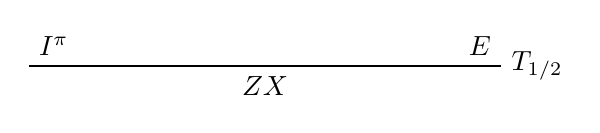
\begin{tikzpicture}
	\draw[thick](0, 0)node[above right]{$I^\pi$}--(6, 0)node[midway, below]{$\nucli ZX$}node[above left]{$E$}node[right]{$T_{1/2}$};
\end{tikzpicture}
\captionof{figure}{能态的描述}
\end{center}
\paragraph{壳层模型}\index{壳层模型}原子的幻数:电子数为$2,10,18,36,54,86$时,元素特别稳定,意味着某些特定壳层的闭合。

核的幻数:质子数或中子数为$2,8,20,28,50,82,126$时,原子核特别稳定,是否也意味着壳层的闭合?

类比原子壳层模型,原子核的壳层结构模型假设:
\begin{compactenum}
	\item 每个能级上容纳的核子数目有一定的限制;
	\item 核子在核内的运动是独立的;

	Pauli原理既限制了每一能级所容纳核子的数目,同时也限制了原子核中核子间的碰撞概率——低能级的核子因碰撞而跃迁到较高能级的概率很小,这使得核子在核内有较大的自由程,单个核子可以在核内“独立运动”。
	\item 核内存在一平均场。

	虽无原子中不变的中心力场,但核子可以看成是在其它核子所形成的平均场中运动;对接近球形的原子核,可以认为这个力场是中心力场。
\end{compactenum}
谐振子势阱各能级的核子数为$2,6,12,20,\ldots$只能给出前三个幻数$2,8,20$,其他许多势阱模型也无法给出更好的结果。

1949年,M. G. Mayer和J. H. D. Jensen在势阱中加入了自旋-轨道耦合项,得到了幻数的关键项。(\nobel{1963})\index{自旋-轨道耦合}

总角动量量子数$j=\ell\pm 1/2$,每个能级上最多放$2j+1$个核子。
\begin{center}
	\captionof{table}{用字母表示轨道角动量}
	\begin{tabular}{cccccccc}
		\toprule
		&s&p&d&f&g&h&$\cdots$\\
		\midrule
		$\ell$&0&1&2&3&4&5&$\cdots$\\
		\bottomrule
	\end{tabular}
\end{center}
由于自旋-轨道耦合,原先1p能级会分裂成1p$_{1/2}$和1p$_{3/2}$两个能级,他们分别能容纳2和4个核子。自旋轨道平行的能级(即$\ell+1/2$)会比反平行(即$\ell-1/2$)能量更低,二者的能量差$\propto 2\ell+1$。
\begin{center}
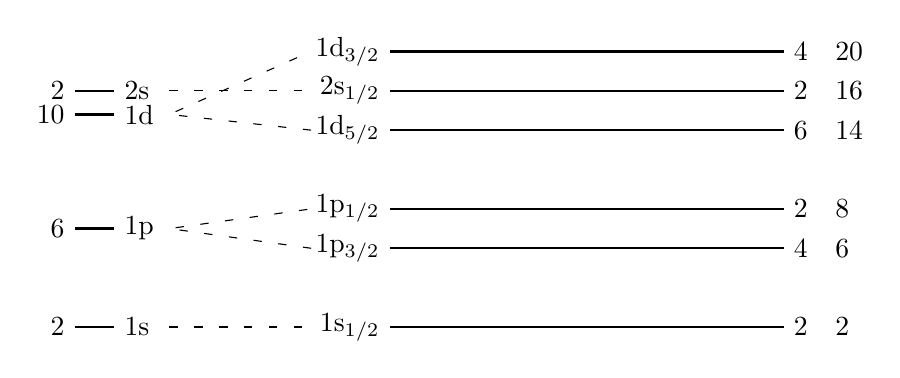
\begin{tikzpicture}
	% 1s
	\draw[thick](-4, 0)node[left]{2}--(-3.5, 0)node[right]{1s};
	\draw[loosely dashed](-2.8, 0)--(-1, 0);
	\draw[thick](0, 0)node[left]{1s$_{1/2}$}--(5, 0)node[right]{2\quad 2};
	% 1p
	\draw[thick](-4, 1.25)node[left]{6}--(-3.5, 1.25)node[right]{1p};
	\draw[loosely dashed](-1, 1)--(-2.8, 1.25)--(-1, 1.5);
	\draw[thick](0, 1)node[left]{1p$_{3/2}$}--(5, 1)node[right]{4\quad 6};
	\draw[thick](0, 1.5)node[left]{1p$_{1/2}$}--(5, 1.5)node[right]{2\quad 8};
	% 1d
	\draw[thick](-4, 2.7)node[left]{10}--(-3.5, 2.7)node[right]{1d};
	\draw[loosely dashed](-1, 2.5)--(-2.8, 2.7)--(-1, 3.5);
	\draw[thick](0, 2.5)node[left]{1d$_{5/2}$}--(5, 2.5)node[right]{6\quad 14};
	\draw[thick](0, 3.5)node[left]{1d$_{3/2}$}--(5, 3.5)node[right]{4\quad 20};
	% 2s
	\draw[thick](-4, 3)node[left]{2}--(-3.5, 3)node[right]{2s};
	\draw[loosely dashed](-2.8, 3)--(-1, 3);
	\draw[thick](0, 3)node[left]{2s$_{1/2}$}--(5, 3)node[right]{2\quad 16};
\end{tikzpicture}
\captionof{figure}{自旋-轨道耦合项引起的能级分裂示意图}
\end{center}
\paragraph{基态核特点}
\begin{compactitem}
	\item 偶偶核中,成对成对核子间角动量方向相反,因此基态偶偶核自旋为0,宇称为$+$;
	\item 奇$A$核中其余偶数个核子的贡献相当于一个偶偶核的贡献,因此模型也叫\textit{单粒子模型}。最后一个奇核子的角动量$j$和轨道量子数$\ell$决定了自旋$j$,宇称$(-)^\ell$;
	\item 奇奇核自旋、宇称由两个奇核子状态决定。
\end{compactitem}

